\documentclass[10pt]{article}
\usepackage[a4paper,landscape,margin=0pt]{geometry}
\usepackage{graphicx}
\usepackage{tikz}
\usepackage{xcolor}
\usepackage[T1]{fontenc}
\usepackage[utf8]{inputenc}
\pagestyle{empty}
\setlength{\parindent}{0pt}

% -----------------------------------------------------------------------------
% Carte de Port Nyanzaru - feuille A4 paysage
% -----------------------------------------------------------------------------
% La page est composee de deux images A5 placees cote a cote :
%   gauche : carte originale + reperes numerotes ;
%   droite : fond parchemin + legende.
%
% Les deux images occupent chacune exactement une moitie de la page :
%   148.5 mm x 210 mm.
%
% Pour deplacer un repere, modifier uniquement les deux nombres de \MapMarker.
% Les coordonnees sont NORMALISEES par rapport a l'image de gauche :
%   x = 0   bord gauche ; x = 1   bord droit
%   y = 0   bord bas    ; y = 1   bord haut
% -----------------------------------------------------------------------------

\definecolor{markerred}{HTML}{A52A2A}
\definecolor{markertext}{HTML}{2B2118}

% Dimensions d'une demi-page A4 paysage = A5 portrait.
\newcommand{\HalfW}{148.5}
\newcommand{\PageH}{210}

% Repere rond sur la carte de gauche.
\newcommand{\MapMarker}[3]{%
  \pgfmathsetmacro{\mx}{(#2)*\HalfW}%
  \pgfmathsetmacro{\my}{(#3)*\PageH}%
  \node[
    circle,
    fill=markerred,
    draw=white,
    line width=0.7pt,
    minimum size=6.8mm,
    inner sep=0pt,
    font=\bfseries\small,
    text=white
  ] at ([xshift=\mx mm,yshift=\my mm]current page.south west) {#1};%
}

% Numero de la legende.
\newcommand{\LegendNumber}[1]{%
  \tikz[baseline=(n.base)]\node[
    circle,
    fill=markerred,
    draw=markertext,
    line width=0.45pt,
    minimum size=6.5mm,
    inner sep=0pt,
    font=\bfseries\small,
    text=white
  ] (n) {#1};%
}

\begin{document}
\begin{tikzpicture}[remember picture,overlay,x=1mm,y=1mm]

  % ---------------------------------------------------------------------------
  % DEUX IMAGES A5 COTE A COTE
  % ---------------------------------------------------------------------------

  % Moitie gauche : carte.
  \node[anchor=south west,inner sep=0pt]
    at (current page.south west)
    {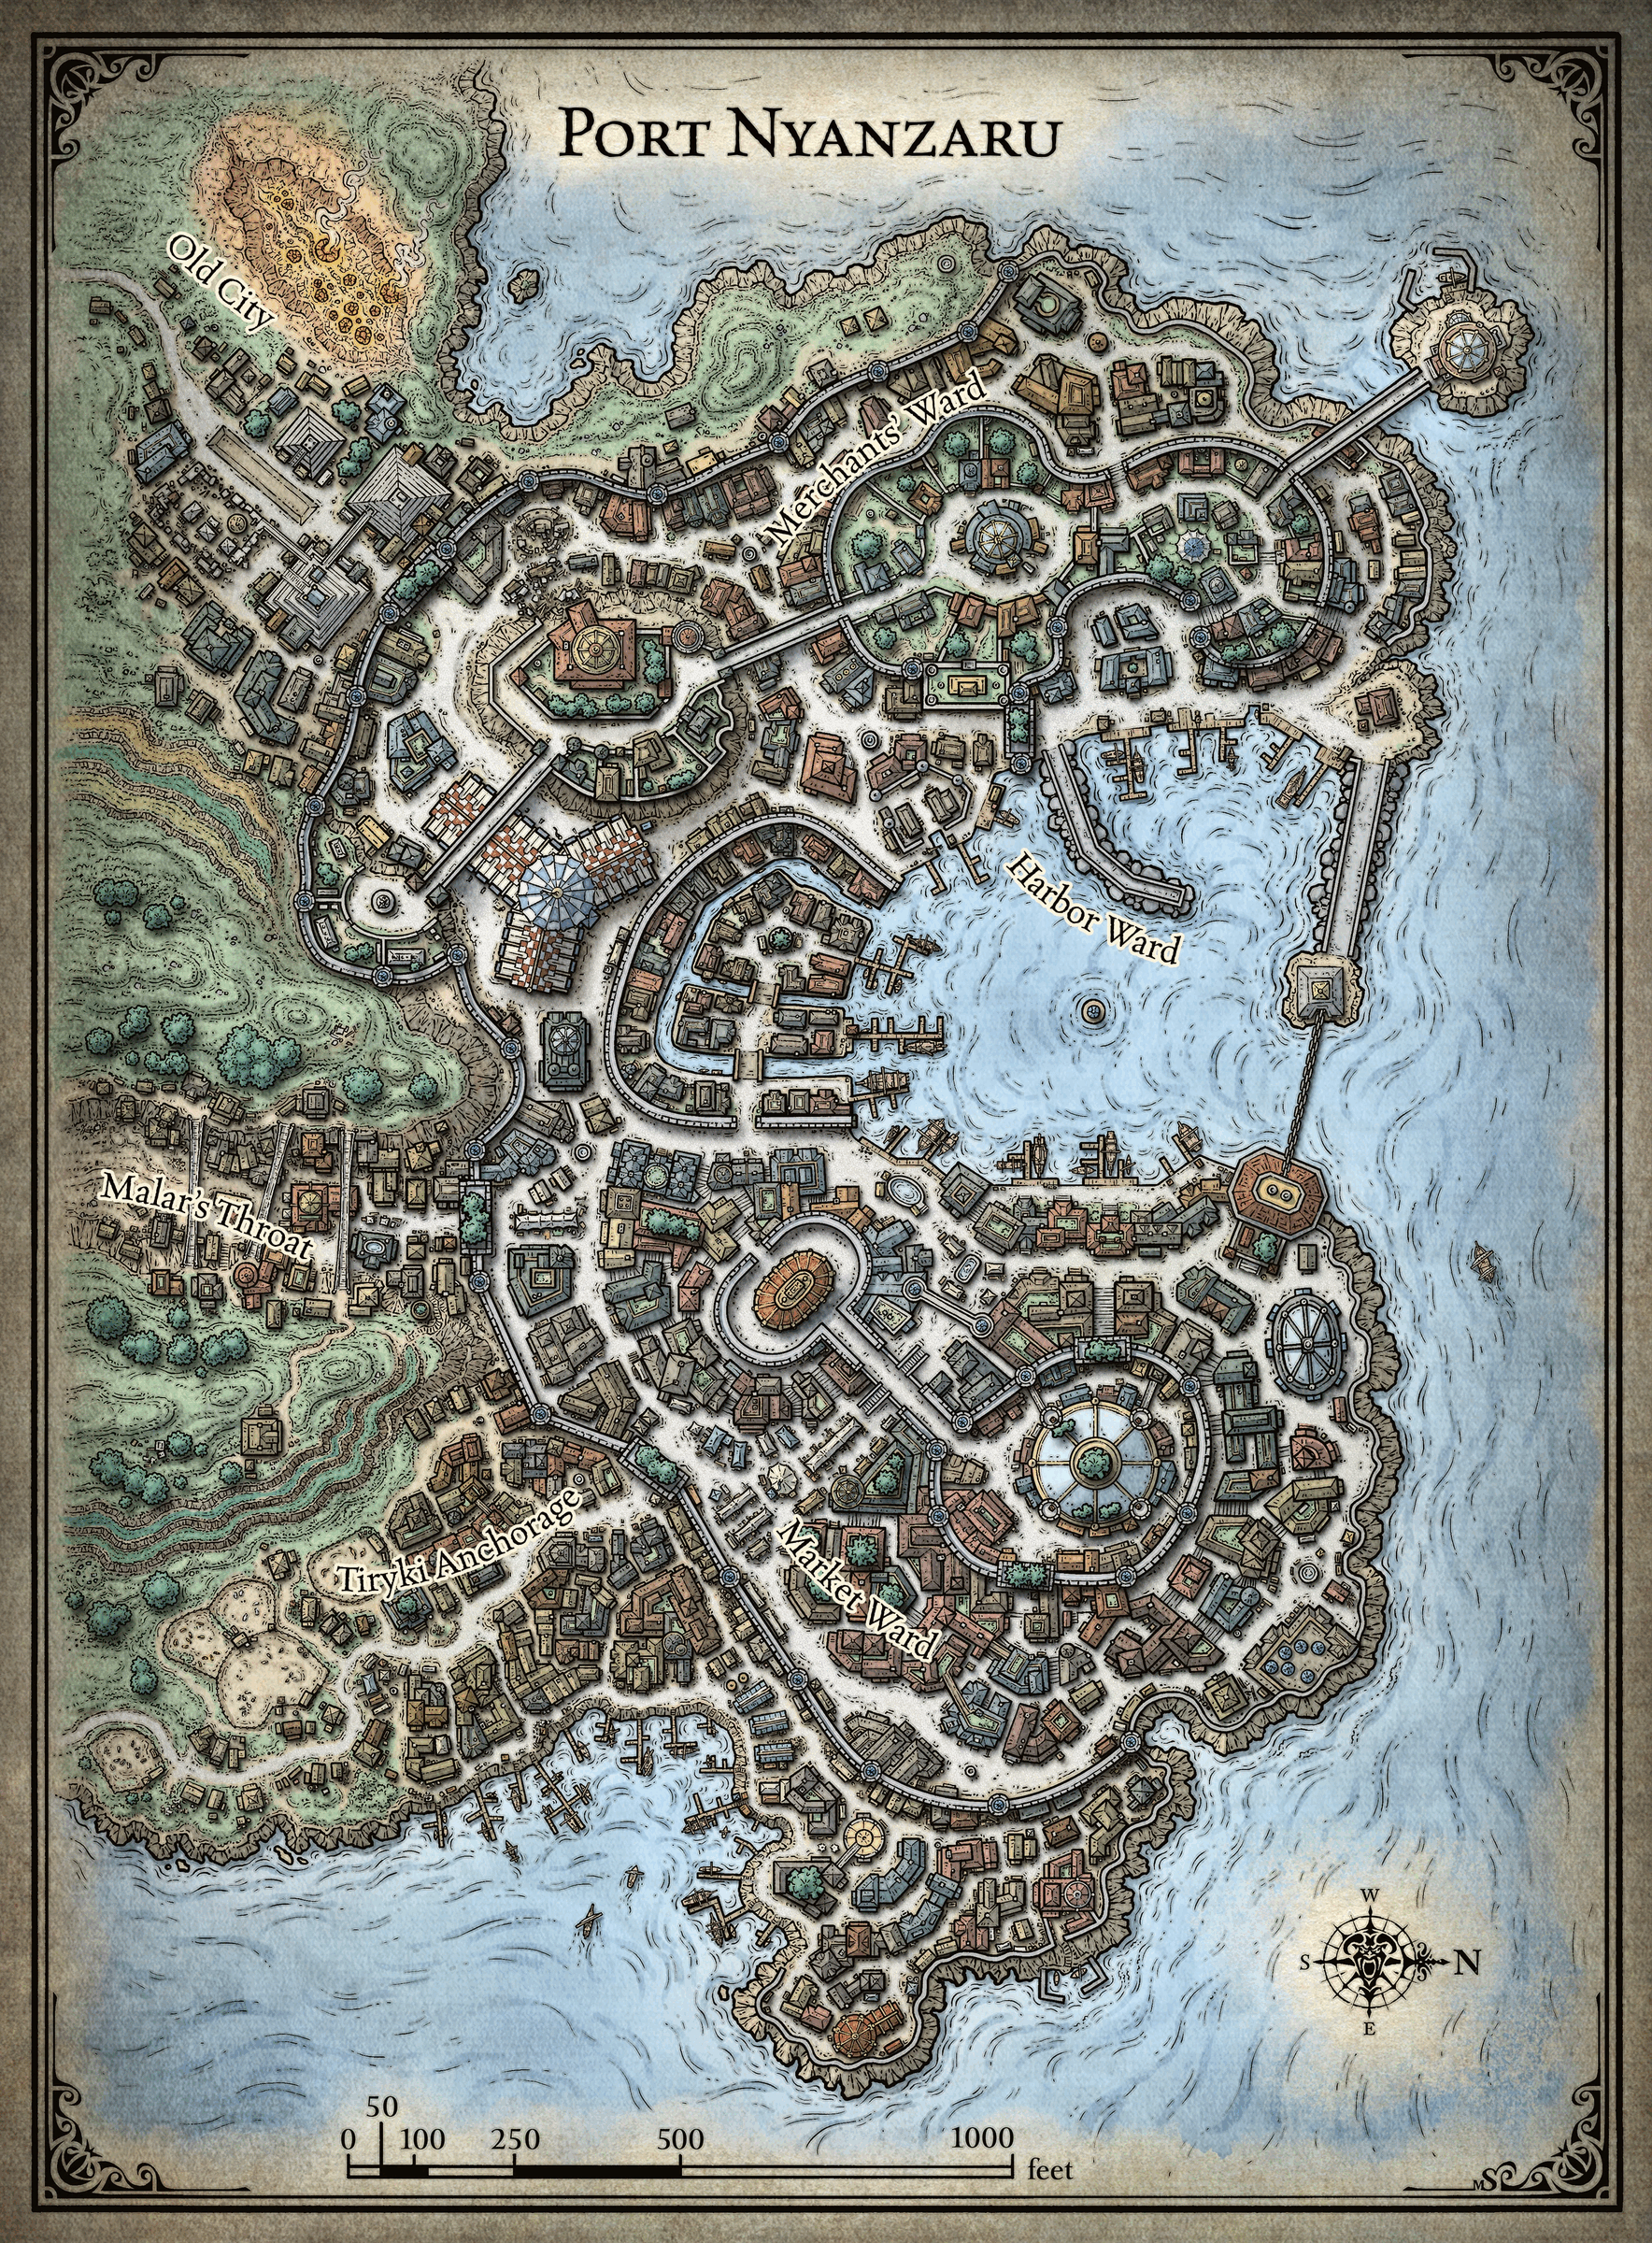
\includegraphics[width=148.5mm,height=210mm]{port_nyanzaru.png}};

  % Moitie droite : parchemin vierge.
  \node[anchor=south west,inner sep=0pt]
    at ([xshift=148.5mm]current page.south west)
    {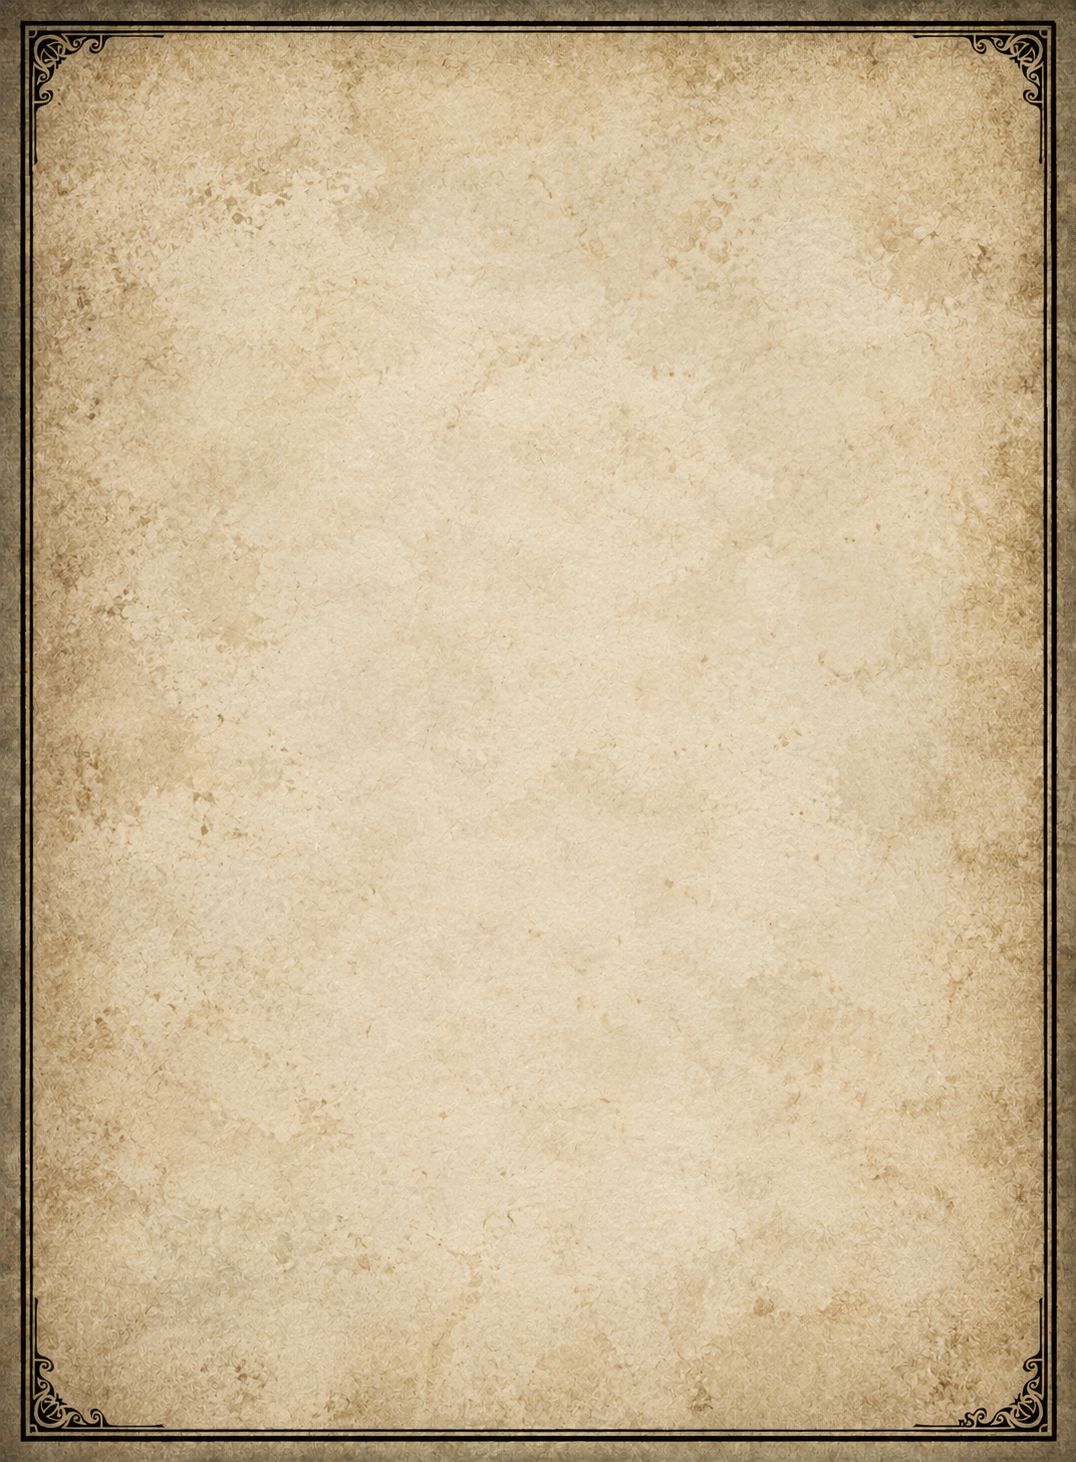
\includegraphics[width=148.5mm,height=210mm]{fond_parchemin.png}};

  % ---------------------------------------------------------------------------
  % REPERES DE LA CARTE
  % Modifier uniquement les deux coordonnees x/y pour ajuster leur position.
  % ---------------------------------------------------------------------------
  \MapMarker{1}{0.73}{0.80} % Maison de Wakanga
  \MapMarker{2}{0.69}{0.72} % Temple de Gond
  \MapMarker{3}{0.37}{0.72} % Palais dore
  \MapMarker{4}{0.34}{0.61} % Grand Bazar / Grand Souk
  \MapMarker{5}{0.44}{0.34} % Marche quotidien
  \MapMarker{6}{0.468}{0.362} % Auberge du Lezard tonnant
  \MapMarker{7}{0.542}{0.284} % Maison de repos de Kaya
  \MapMarker{8}{0.834}{0.692} % Capitainerie

  % ---------------------------------------------------------------------------
  % LEGENDE SUR LE PARCHEMIN DE DROITE
  % ---------------------------------------------------------------------------

  \node[anchor=north west,text=markertext,font=\bfseries\LARGE]
    at ([xshift=158mm,yshift=191mm]current page.south west)
    {Port Nyanzaru};

  \node[anchor=north west,text=markertext!80,font=\itshape\small]
    at ([xshift=158mm,yshift=181mm]current page.south west)
    {Lieux decouverts par le groupe};

  \node[anchor=west,text=markertext,font=\large]
    at ([xshift=158mm,yshift=165mm]current page.south west)
    {\LegendNumber{1}\hspace{2mm} Maison de Wakanga};

  \node[anchor=west,text=markertext,font=\large]
    at ([xshift=158mm,yshift=153mm]current page.south west)
    {\LegendNumber{2}\hspace{2mm} Temple de Gond};

  \node[anchor=west,text=markertext,font=\large]
    at ([xshift=158mm,yshift=141mm]current page.south west)
    {\LegendNumber{3}\hspace{2mm} Palais dore};

  \node[anchor=west,text=markertext,font=\large]
    at ([xshift=158mm,yshift=129mm]current page.south west)
    {\LegendNumber{4}\hspace{2mm} Grand Bazar / Grand Souk};

  \node[anchor=west,text=markertext,font=\large]
    at ([xshift=158mm,yshift=117mm]current page.south west)
    {\LegendNumber{5}\hspace{2mm} Marche quotidien / Bazar rouge};

  \node[anchor=west,text=markertext,font=\large]
    at ([xshift=158mm,yshift=105mm]current page.south west)
    {\LegendNumber{6}\hspace{2mm} Auberge du Lezard tonnant};

  \node[anchor=west,text=markertext,font=\large]
    at ([xshift=158mm,yshift=93mm]current page.south west)
    {\LegendNumber{7}\hspace{2mm} Maison de repos de Kaya};

  \node[anchor=west,text=markertext,font=\large]
    at ([xshift=158mm,yshift=81mm]current page.south west)
    {\LegendNumber{8}\hspace{2mm} Capitainerie};

\end{tikzpicture}
\null
\end{document}
